
\subsection{Matrix Multiplication}

\begin{figure}[H]
  \begin{center}
    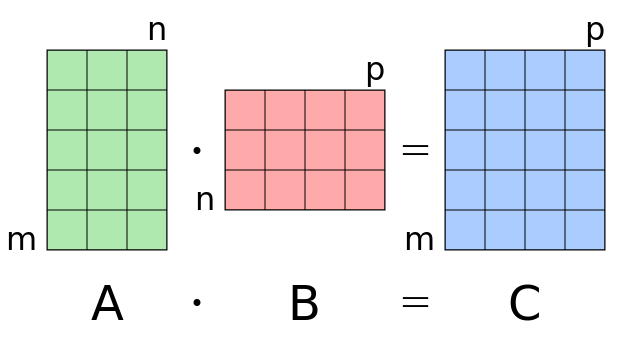
\includegraphics[width=0.15\textwidth]{media/Matrix_multiplication_qtl1.png}
  \end{center}
\end{figure}

Let \( A \in \mathbb{R}^{n \times m} \) and \( B \in \mathbb{R}^{m \times c} \). The product \( C = AB \in \mathbb{R}^{n \times m} \) is defined as:

\begin{equation}
  c_{ij} = \sum_{k=1}^{m} a_{ik} b_{kj}
\end{equation}

For \( i = 1, \ldots, n \) and \( j = 1, \ldots, m \).

For matrix multiplication, the number of \textbf{columns in the first matrix} must be equal to the number of \textbf{rows in the second matrix}. The result matrix has the number of \textbf{rows of the first} and the number of \textbf{columns of the second matrix}.

Matrix multiplication is associative and distributive, but not commutative: \( AB \neq BA \) in general.
